%=======================================================
% CHAPTER 3: APPLICATIONS
%=======================================================

%--- Section Title Frame ---
\begin{frame}[plain]
  \begin{center}\bfseries\centering
    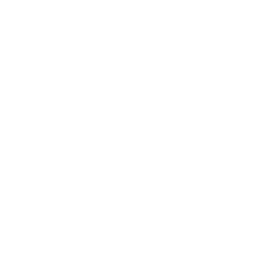
\includegraphics[scale=1]{assets/branding/opa0}
    \vspace{-5.75cm}\\
    {\adjustbox{scale=2.3}{\color{TealDarkCyan}\;IV.\;Applications}}
    \bigskip\bigskip
    {\ }\vspace{4cm}\\
    \bigskip
  \end{center}
\end{frame}

%--- Slide: CRC ---
\begin{frame}{\textbf{IV. Applications}}{CRC --- Cyclic Redundancy Check}

\begin{columns}[T]
  \begin{column}{.55\textwidth}
    \defbox[Principle]{
    \small Transmit $c(X) = m(X)\,g(X)$.\\
    Receiver computes $v(X)\bmod g(X)$:
    \begin{itemize}
      \item $= 0$: no error detected
      \item $\neq 0$: error detected
    \end{itemize}
    }

    \medskip
    \textbf{Hardware advantage (LFSR):}
    \begin{itemize}\small
      \item Only $r = \deg g$ flip-flops needed
      \item One bit processed per clock cycle
      \item Near-zero latency, no buffering
    \end{itemize}

    \medskip
    \textbf{vs.\ general linear codes:}\\
    {\small Must store $k\times n$ matrix and perform $kn$ multiplications per block.}
  \end{column}
  \begin{column}{.42\textwidth}
    \textbf{Standard polynomials:}
    \medskip
    \renewcommand{\arraystretch}{1.3}
    \begin{tabular}{@{}lll@{}}
      \toprule
      Name & $r$ & Used in\\
      \midrule
      CRC-8  & 8  & sensors, I$^2$C\\
      CRC-16 & 16 & USB, MODBUS\\
      CRC-32 & 32 & Ethernet, ZIP\\
      CRC-64 & 64 & ISO, ECMA\\
      \bottomrule
    \end{tabular}

    \medskip\small
    \textbf{CRC-32} (Ethernet):
    \[\small g(X)=X^{32}+X^{26}+X^{23}\]
    \[+X^{22}+X^{16}+X^{12}+\cdots+1\]
  \end{column}
\end{columns}
\end{frame}

%--- Slide: Reed-Solomon and BCH ---
\begin{frame}{\textbf{IV. Applications}}{BCH Codes and Reed--Solomon Codes}

\begin{columns}[T]
  \begin{column}{.50\textwidth}
    \defbox[BCH Codes]{
    \small Cyclic codes over $\F_q$ with \emph{designed distance} $\delta$, via consecutive roots in $\F_{q^m}$. Binary BCH codes are industry workhorses.
    \begin{itemize}
      \item \textbf{Flash memory}: $[2047,1989]$ BCH
      \item \textbf{Satellite comm.}: high correction $t$
    \end{itemize}
    }

    \medskip
    \defbox[Reed--Solomon Codes]{
    \small Nonbinary cyclic MDS codes with $d_{\min} = n-k+1$ (optimal!). Correct bursts of symbol errors.
    \begin{itemize}
      \item \textbf{CD/DVD/Blu-ray}: $[255,223]_{256}$ RS\\
            corrects 16 byte-errors per block
      \item \textbf{QR codes}: RS over $\F_{2^8}$
      \item \textbf{Deep-space}: Voyager, Mars Rover
    \end{itemize}
    }
  \end{column}
  \begin{column}{.47\textwidth}
    \textbf{Why Reed--Solomon codes are special:}

    \medskip
    \begin{tikzpicture}[
      tbox/.style={draw,rounded corners,thick,align=center,minimum height=.7cm},
      arr/.style={-Stealth,thick,TealDarkCyan}
    ]
      \node[tbox, fill=TealDarkCyan!15, minimum width=5cm] (q1)
        {\small $n-k+1$ is the Singleton bound};
      \node[tbox, fill=orange!15, below=.5cm of q1, minimum width=5cm] (q2)
        {\small RS achieves it: \textbf{MDS code}};
      \node[tbox, fill=TealDarkCyan!25, below=.5cm of q2, minimum width=5cm] (q3)
        {\small Maximum error correction for the rate};
      \draw[arr] (q1)--(q2);
      \draw[arr] (q2)--(q3);
    \end{tikzpicture}

    \medskip\small
    \textbf{Decoding:} Berlekamp--Massey algorithm (1968) solves the error-locator polynomial in $O(n^2)$ operations.
  \end{column}
\end{columns}
\end{frame}

%--- Slide: Post-Quantum Cryptography ---
\begin{frame}{\textbf{IV. Applications}}{Post-Quantum Cryptography: HQC}

\begin{columns}[T]
  \begin{column}{.55\textwidth}
    \defbox[Quasi-Cyclic Codes]{
    \small A code closed under an $\ell$-step cyclic shift ($\ell > 1$). Generator and parity-check matrices consist of \textbf{circulant blocks}:
    \[C = \begin{bmatrix}1&0&1&1\\1&1&0&1\\1&1&1&0\\0&1&1&1\end{bmatrix}\]
    {\footnotesize Each row is a cyclic shift of the previous one. Determined by its \textbf{first row alone}.}
    }
  \end{column}
  \begin{column}{.42\textwidth}
    \defbox[HQC (NIST PQC, 2025)]{
    \small \textbf{Hamming Quasi-Cyclic} key encapsulation:
    \begin{enumerate}\small
      \item Keys are polynomials in $\F_2[X]/\ideal{X^n-1}$
      \item Arithmetic via polynomial multiplication
      \item Security: \textbf{syndrome decoding} is NP-hard
    \end{enumerate}
    }

    \medskip
    \textbf{Why quasi-cyclic?}
    \begin{itemize}\small
      \item McEliece (1978): secure but MB-size keys
      \item QC structure: circulant $\to$ 1 polynomial $\to$ compact keys
      \item Fast NTT-based arithmetic
    \end{itemize}
  \end{column}
\end{columns}

\medskip
\begin{center}
\begin{tikzpicture}[
  ubox/.style={draw,rounded corners,thick,align=center,minimum height=.65cm,minimum width=2.8cm},
  arr/.style={-Stealth,thick,TealDarkCyan}
]
  \node[ubox, fill=gray!20]          (cc)  {Cyclic codes};
  \node[ubox, fill=TealDarkCyan!20, right=.8cm of cc]  (qc)  {Quasi-cyclic codes};
  \node[ubox, fill=orange!20,       right=.8cm of qc]  (hqc) {HQC};
  \draw[arr] (cc) -- (qc)  node[midway,above]{\tiny $\ell$-shift};
  \draw[arr] (qc) -- (hqc) node[midway,above]{\tiny + hardness};
\end{tikzpicture}
\end{center}
\end{frame}

%--- Slide: Summary ---
\begin{frame}{\textbf{IV. Applications}}{Summary and Perspective}

\begin{columns}[T]
  \begin{column}{.48\textwidth}
    \renewcommand{\arraystretch}{1.3}
    \begin{tabular}{@{}p{1.5cm}p{1.8cm}p{2.5cm}@{}}
      \toprule
      \textbf{Era} & \textbf{Direction} & \textbf{Key idea}\\
      \midrule
      1950s & Engineering $\to$ algebra & Cyclic shift $=$ ideal\\[2pt]
      1960s--70s & Algebra $\to$ design & BCH bound, RS codes\\[2pt]
      1990s--now & Integration & Hardware, crypto\\
      \bottomrule
    \end{tabular}
  \end{column}
  \begin{column}{.48\textwidth}
    \defbox[The Big Picture]{
    \small
    \begin{itemize}
      \item \textbf{Linear codes}: rich algebraic structure
      \item \textbf{Cyclic codes}: polynomial ring $\F_q[X]/\ideal{X^n-1}$, ideals, LFSR circuits
      \item \textbf{BCH / RS}: designed distance, optimal rate
      \item \textbf{Quasi-cyclic}: compact keys for post-quantum security
    \end{itemize}
    }
  \end{column}
\end{columns}

\bigskip
\begin{alertblock}{Closing Thought}
\centering\small
Abstract algebra is not separate from engineering — in coding theory, \textbf{ring theory} and \textbf{shift-register circuits} are two faces of the same mathematics.
\end{alertblock}
\end{frame}
